\chapter{Mô hình đề xuất cho giải pháp thương mại điện tử trong mạng xã hội}

\section{Tổng quan}

Từ những nghiên cứu, quan sát và tổng hợp như trên, chúng tôi đề xuất một mô hình thương mại xã hội có khả năng tổng hợp những ưu điểm của nhiều hệ thống khác nhau để giải quyết yếu điểm của những hệ thống còn lại. Mô hình này bao gồm 2 hệ thống hoạt động song song trên cùng một nền tảng, vừa hỗ trợ các tính năng của mạng xã hội trực tuyến, vừa cung cấp giải pháp thương mại điện tử mà cụ thể là hình thức thương mại B2C và C2C.



\section{Lược đồ Usecases và Mô tả chi tiết}
\subsection{Lược đồ Usecases}

\begin{figure}[H]
	\centering
	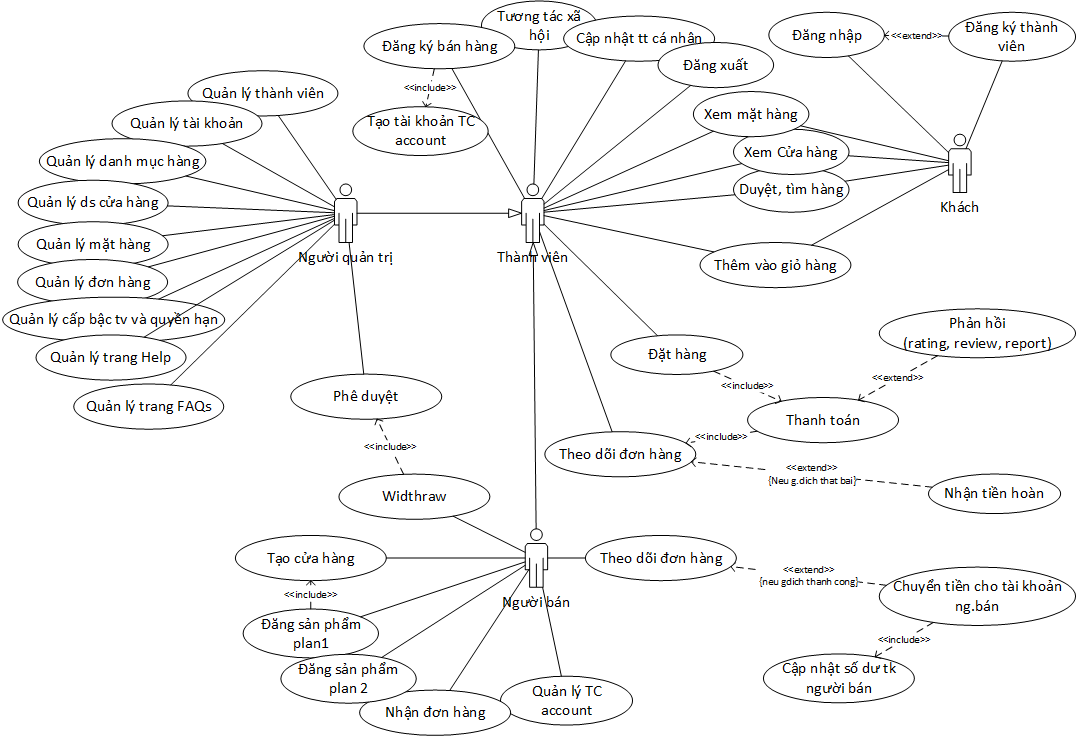
\includegraphics[width=1\textwidth]{img/usecase-diagram.PNG} 
	\caption{Lược đồ Usecases}
\end{figure}
(Sửa lai: thêm vào giỏ hàng, Bỏ include chỗ theo dõi đơn hàng và thanh toán, thêm extend chỗ phản hồi/thanh toán, quản lí mặt hàng => quản lý sản phẩm)

\subsection{Phân cấp, phân loại người dùng}
\begin{enumerate}
	\item Khách: Người dùng chưa đăng nhập hệ thống
	\item Thành viên: Người dùng đã đăng nhập hệ thống
	\begin{enumerate}
		\item Người quản trị: Thành viên có cấp bậc Administrator
		\item Thành viên thông thường
		\item Thành viên đăng ký bán hàng (Seller): Bất cứ thành viên nào (admin hoặc thành viên thông thường) đã đăng ký Seller
	\end{enumerate}
\end{enumerate}

\subsection{Danh sách các Usecase}
\begin{table}[H]
	\centering
	\begin{tabularx}{\textwidth}{|l|>{\raggedright\arraybackslash}X|>{\raggedright\arraybackslash}X |}
		\hline
		
		Tên Usecase &Actor &Mô tả\\
		\hline
		
		Đăng ký thành viên&Khách&Đăng ký tài khoản thành viên\\
		\hline	
		
		Đăng nhập&Khách&Đăng nhập vào hệ thống bằng tài khoản thành viên\\
		\hline
		
		Đăng xuất&Thành viên&Đăng xuất khỏi hệ thống\\
		\hline
		
		Quản lí thông tin cá nhân&Thành viên&Xem và chỉnh sửa thông tin cá nhân, ảnh đại diện\\
		\hline
		
		Tương tác xã hội&Thành viên&Thực hiện các hành vi của mạng xã hội trực tuyến như kết bạn, chia sẻ nội dung số, "thích" một nội dung nào đó,...\\
		\hline
		
		Xem hàng hoá&Khách, Thành viên&Duyệt, tìm kiếm hàng, xem chi tiết mặt hàng\\
		\hline
		
		 Đăng Ký bán hàng&Thành viên&Đăng ký để bán hàng trong MXH, sau khi đăng ký bán hàng, thành viên có tài khoản seller (TradersClub account)\\
		 \hline
		 
		 Thêm vào giỏ hàng&Khách, Thành viên&Thêm hàng vào giỏ hàng\\
		 \hline
		 
		 Đặt hàng&Thành viên&Đặt mua tất cả hàng theo số lượng đã thêm vào giỏ hàng\\
		 \hline
		 
		 Theo dõi đơn hàng&Thành viên&Xem trạng thái đơn hàng, chọn xác nhận sau khi nhận được hàng\\
		 \hline
		 
		 Theo dõi đơn hàng&Người bán&Xem trạng thái đơn hàng, cập nhật tình trạng đơn hàng sau khi giao hàng thành công\\
		 \hline
		 
		 Quản lý TC Account&Người bán&Xem và quản lý thông tin tài khoản, số dư tài khoản...\\
		 \hline
		 
		 Tạo cửa hàng (Stall)&Người bán&Người bán tạo và quản lý của hàng của mình\\ \hline
		 
		 Đăng sản phẩm - plan 1&Người bán&Đăng sản phẩm trong cửa hàng đã tạo\\
		 \hline
		 
		 Đăng sản phẩm - plan 2&Người bán&Đăng sản phẩm riêng lẻ, không cần tạo cửa hàng\\ \hline
		 
		Nhận đơn hàng - plan 1&Người bán&Cập nhật danh sách đặt hàng của món hàng đã tạo theo plan 1\\ \hline
		
		Nhận đơn hàng - plan 2&Người bán&Cập nhật danh sách đặt hàng của món hàng đã tạo theo plan 2\\ \hline
		
		Rút tiền (Withdraw)&Người bán&Rút tiền từ tài khoản người bán về tài khoản Paypal\\ \hline
		
		Quản lí thành viên&Quản trị viên&Xem danh sách toàn bộ thành viên trong hệ thống và thực hiện một số tác vụ liên quan\\ \hline
		
		Quản lí tài khoản&Quản trị viên&Xem danh sách toàn bộ tài khoản bán hàng trong hệ thống và thực hiện một số tác vụ liên quan\\ \hline
		
		Quản lý danh mục hàng&Quản trị viên&Xem, tạo thêm và chỉnh sửa các danh mục hàng\\ \hline
		
		Quản lí cửa hàng&Quản trị viên&Xem danh sách toàn bộ cửa hàng đã được tạo trong hệ thống và thực hiện một số tác vụ liên quan\\ \hline
				
		Quản lý sản phẩm&Quản trị viên&Xem danh sách toàn bộ sản phẩm đã được tạo trong hệ thống và thực hiện một số tác vụ liên quan\\ \hline
		
		Quản lý đơn hàng&Quản trị viên&Xem danh sách toàn bộ đơn hàng đã được tạo trong hệ thống và thực hiện một số tác vụ liên quan\\ \hline
		
		Quản lí thành viên&Quản trị viên&Quản lí cấp bậc thành viên và quyền hạn của mỗi cấp\\ \hline
		
		Quản lý trang Help&Quản trị viên&Xây dựng và cập nhật các hướng dẫn\\ \hline
		
		Quản lí trang FAQs&Quản trị viên&Cập nhật, thêm các FAQ\\ \hline
		
		Phê duyệt&Quản trị viên&Phê duyệt các yêu cầu rút tiền từ các TC account\\ \hline
	\end{tabularx}
	\caption{Danh sách các Usecase}
\end{table}

\subsection{Đặc tả các Usecases}

\subsubsection{Đăng ký thành viên}
\begin{enumerate}
	\item Pre-Condition\\
	Không có.
	\item Post-Condition\\
	Hệ thống tạo mới một tài khoản trong CSDL và yêu cầu người dùng xác thực qua email trong vòng 3 ngày.
	\item Triggers
	\begin{enumerate}
		\item Người dùng truy cập vào hệ thống nhưng chưa đăng nhập
	\end{enumerate}
	\item Basic flow
	\begin{enumerate}
		\item Khách chọn "Sign Up" trên mini menu.
		\item Nhập thông tin tài khoản: Email, Password, Password again, url address, Accept term \& condition sau đó chọn "Craate account".
		\item Nhập thông tin cá nhân: Lname, Fname, Birthday, About me
		\item Upload ảnh đại diện hoặc bỏ qua bước này.
		\item Thông báo thành công và chuyển đến trang Profile.
		\item Người dùng xác thực tài khoản bằng email.
	\end{enumerate}
	\item Alternative flow
	\item Business rule
	\begin{enumerate}
		\item Nếu email đã sử dụng hoặc mật khẩu không hợp lệ: Thông báo lỗi và yêu cầu nhập lại.
		\item Thiếu thông tin Lname, Fname: Báo lỗi và yêu cầu nhập Lname, Fname.
		\item Kích thước hình ảnh không phù hơp: báo lỗi và yêu cầu người dùng chọn hình ảnh khác.
	\end{enumerate}
\end{enumerate}

\subsubsection{Đăng nhập hệ thống}
\begin{enumerate}
	\item Pre-Condition\\
	Người sử dụng đã có tên truy cập và mật khẩu hợp lệ được lưu trong cơ sở dữ liệu.
	\item Post-Condition\\
	Hệ thống xác thực và đưa người sử dụng đến trang chính.
	\item Triggers
		\begin{enumerate}
			\item Người dùng chưa đăng nhập hệ thống
			\item Người dùng chọn "Đăng nhập"
		\end{enumerate}
	\item Basic flow
	\begin{enumerate}
		\item Khách chọn "Sign In" trên mini menu.
		\item Người dùng nhập thông tin “Email và Password” đã đăng ký trước đó
		\item Hệ thống xác thực “email” và “password” mà người dùng vừa nhập.
		\item Hệ thống xác thực thành công và đưa người dùng đến trang chủ của hệ thống.
		\item Xác thực không thành công: Thông báo lỗi và yêu cầu nhập lại.
	\end{enumerate}
	\item Alternative flow\\
	Người dùng chọn "Forgot password" trong trang đăng nhập:
	\begin{enumerate}
		\item Hệ thống hướng dẫn người dùng điền “email” của người dùng
		\item Hệ thống xác thực email đó có tồn tại trong hệ thống hay chưa. Nếu chưa hệ thống sẽ đề nghị người dùng nhập lại
		\item Hệ thống sẽ gửi một email xác thực thay đổi mật khẩu thông qua email người dùng vừa nhập.
		\item Người dùng theo đường link hệ thống gửi trong email và theo hướng dẫn nhập mật khẩu mới.
	\end{enumerate}
	\item Busines Rule
\end{enumerate}

\subsubsection{Đăng xuất hệ thống}
\begin{enumerate}
	\item Pre-Condition\\
	Người dùng đang đăng nhập hệ thống.
	\item Post-Condition\\
	Người dùng đăng xuất hoàn toàn khỏi hệ thống.
	\item Triggers
	\item Basic flow
	\begin{enumerate}
		\item Người dùng chọn "Sign out" trên mini Menu.
		\item Chuyển về trang Landing.
	\end{enumerate}
	\item Alternative flow
	\item Business rule
\end{enumerate}

\subsubsection{Chỉnh sửa thông tin cá nhân}
\begin{enumerate}
	\item Pre-Condition\\
	Người sử dụng đã đăng nhập vào hệ thống.
	\item Post-Condition\\
	Hệ thống cập nhật thông tin mà người dùng thay đổi trong CSDL.
	\item Triggers
	Người dùng đang ở trang “My Profile” và nhấn vào menu “Edit My Profile”.
	\item Basic flow
	\begin{enumerate}
		\item Hệ thống sẽ hiển thị form chỉnh sửa thông tin cá nhân cho thành viên.
		\item Sau khi điền thông tin người dùng nhấn “Lưu lại”.
		\item Hệ thống sẽ kiểm tra tính hợp lệ dữ liệu nhập vào của người dùng. 
		\item Hệ thống lựu lại những thông tin người dùng vừa thay đổi và thông báo cho người dùng đã cập nhật thành công. Trang web sẽ tự động chuyển hướng đến “My Profile”.
	\end{enumerate}
	\item Alternative flow
	\item Business rule
	Nếu dữ liệu người dùng nhập vào không hợp lệ. Hệ thống chỉ ra những thông tin không hợp lệ và yêu cầu người dùng nhập lại những thông tin chưa hợp lệ đó.
\end{enumerate}

\subsubsection{Tương tác xã hội}
\begin{enumerate}
	\item Pre-Condition\\
	Người sử dụng đã đăng nhập vào hệ thống.
	\item Post-Condition\\
	Hệ thống sẽ hiển thị những thao tác thành viên vừa mới thực hiện lên Activity Feed và gửi Notification cho đối tượng mà thao tác đó ảnh hưởng tới (nếu có).
	\item Triggers
	Thành viên ở trang Activity Feed và nhấn vào nút like/share/comment trên một status, comment, post của một thành viên khác trên hệ thống. 
	Thành viên ở trang Activity Feed và post một status/ upload photo/ upload video.
	\item Basic flow
	\begin{enumerate}
		\item Thành viên like/ share/ comment một status/ comment/ post của một thành viên khác trên hệ thống hoặc đăng một status/ upload photo/ video lên trang Activity Feed của hệ thống.
		\item Hệ thống sẽ xử lý những thao tác trên. Nếu mọi thứ hợp lệ, hệ thống sẽ tạo một feed lên trên Activity Feed đồng thời gửi Notification cho đối tượng mà thao tác đó ảnh hưởng tới (nếu có).
	\end{enumerate}
	\item Alternative flow
	\item Business rule
	Tạo 1 activity tương ứng mỗi khi có 1 thực thể mới được tạo ra.
	Gửi thông báo và email đến những thành viên có liên quan với hành động được thực hiện.
\end{enumerate}

\subsubsection{Duyệt tìm trong Marketplace}
\begin{enumerate}
	\item Pre-Condition\\
	Người dùng truy cập vào hệ thống.
	\item Post-Condition\\
	Màn hình hiển thị các danh sách cửa hàng (Stalls) và mặt hàng (Products) tuỳ theo nội dung tìm kiếm.
	\item Triggers
	\begin{enumerate}
		\item Người dùng chọn "Shop" trên Menu chính để truy cập vào Market place.
		\item Người dùng nhấp vào một "post" liên quan đến cửa hàng hoặc mặt hàng trên Newsfeed.
	\end{enumerate}
	\item Basic flow
	\begin{enumerate}
		\item Người dùng chọn "View more" trên các widget liên quan đến cửa hàng mặt hàng hoặc\\
		Người dùng nhấp vào một Category trong Categories widget hoặc\\
		Người dùng nhâp các thông tin tìm kiếm (keyword, mức giá, vị trí) trong Search widget và chon "Search".
		\item hệ thống tìm và hiển thị các nội dung tương ứng.
	\end{enumerate}
	\item Alternative flow
	\item Business rule
\end{enumerate}

\subsubsection{Xem trang chủ của cửa hàng (Stall home)}
\begin{enumerate}
	\item Pre-Condition\\
	Người dùng truy cập vào hệ thống.
	\item Post-Condition\\
	Màn hình hiển thị trang chủ của cửa hàng.
	\item Triggers
	\begin{enumerate}
		\item Người dung nhấp vào một liên kết đến cửa hàng
	\end{enumerate}
	\item Basic flow
	\begin{enumerate}
		\item Người dùng nhấp vào môt liên kết đến cửa hàng.
		\item Màn hình hiển thị trang chủ cửa hàng.
	\end{enumerate}
	\item Alternative flow
	\item Business rule
	Người dùng có thể thực hiện các tương tác đối với cửa hàng: Like, Share, Post, Comment.
\end{enumerate}

\subsubsection{Xem chi tiết mặt hàng}
\begin{enumerate}
	\item Pre-Condition\\
	Người dùng truy cập vào hệ thống.
	\item Post-Condition\\
	Màn hình hiển thị trang thông tin chi tiết mặt hàng.
	\item Triggers
	\begin{enumerate}
		\item Người dung nhấp vào một liên kết đến mặt hàng.
	\end{enumerate}
	\item Basic flow
	\begin{enumerate}
		\item Người dùng nhấp vào môt liên kết đến mặt hàng.
		\item Màn hình hiển thị trang thông tin chih tiết mặt hàng.
	\end{enumerate}
	\item Alternative flow
	\item Business rule
	Người dùng có thể thực hiện các tương tác đối với mặt hàng: Like, Share, Post, Comment.
\end{enumerate}

\subsubsection{Thêm mặt hàng vào giỏ hàng}
\begin{enumerate}
	\item Pre-Condition\\
	Người dùng truy cập vào hệ thống.
	\item Post-Condition\\
	Mặt hàng được thêm vào giỏ hàng.
	\item Triggers
	\item Basic flow
	\begin{enumerate}
		\item Người dùng nhập số lượng muốn mua.
		\item Người dùng chọn "Add to bag" trong trang chi tiết mặt hàng.
		\item Hệ thống hiển thị thông báo thêm thành công trên hộp thoại.
		\item Người dùng chọn "OK" để xác nhận và đóng hộp thoại.
	\end{enumerate}
	\item Alternative flow
	\begin{enumerate}
		\item Người dùng chọn "Add to bag" tương ứng với mặt hàng trên các trang Listing.
		\item Hệ thống thêm tự động mặt hàng được chọn vào giỏ hàng với số lượng mặc định là 1.
		\item Hệ thống hiển thị thông báo thêm thành công trên hộp thoại.
		\item Người dùng chọn "OK" để xác nhận và đóng hộp thoại. 
	\end{enumerate}	
	\item Business rule
\end{enumerate}

\subsubsection{Đặt hàng}
\begin{enumerate}
	\item Pre-Condition\\
	Phải có ít nhất 1 mặt hàng trong giỏ hàng.
	\item Post-Condition\\
	Đơn hàng được lưu vào CSDL, người mua, người bán đề có thể theo dõi tình trạng đơn hàng.
	\item Triggers
	Người dùng nhấn chon "Check Out" trong giỏ hàng.
	\item Basic flow
	\begin{enumerate}
		\item Người dùng chon "Check Out" từ giỏ hàng.
		\item Nếu người dùng đã đăng nhập, chuyển đến trang Shipping Infomation yêu cầu điền thông tin tên, số điện thoại và địa chỉ người nhận.
		\item Nếu người dùng là khách, hiện hộp thoại đăng nhập. Sau khi đăng nhập thành công chuyển đến trang Shipping Infomation.
		\item Sau khi điền thông tin người nhận, chuyển đến trang thanh toán. 
		\item Thanh toán thành công, trở lại trang Home.
	\end{enumerate}
	\item Alternative flow
	\item Business rule
	\begin{enumerate}
		\item Gửi email xác nhận thông tin và mã đơn hàng cho người đặt hàng.
		\item Gửi email và feed notification cho người bán.
		\item Tiền thanh toán thông qua Payment Gateway sẽ được chuyển đến tài khoản hệ thống trước khi giao dịch hoàn tất.
	\end{enumerate}
\end{enumerate}

\subsubsection{Theo dõi và hoàn tất đơn hàng - Người mua}
\begin{enumerate}
	\item Pre-Condition\\
	Người mua đã đặt hàng và thanh toán thành công.
	\item Post-Condition\\
	Tiền mua hàng chuyển vào tài khoản người bán hoặc được hoàn trả cho người mua. Trạng thái đơn hàng chuyển thành "Complete".
	\item Triggers\\
	Người dùng nhấp chọn liên kết đến đơn hàng.
	\item Basic flow
	\begin{enumerate}
		\item Người dùng xem lại đơn hàng. Nếu trạng thai đơn hàng là "Shipped", người mua thấy button "Received".
		\item Chọn "Received": đơn hàng chuyển trạng thái thành "Completed".
		\item Hệ thống cập nhật (tăng) số dư tài khoản người bán sau tương ứng số tiền bán hàng - commission.
		\item Seller nhận được notification thông báo giao dịch thành công.
	\end{enumerate}
	\item Alternative flow\\
	Người mua không xác nhận "Received":
	\begin{enumerate}
		\item Nếu trạng thái đã chuyển thành "Shipped" mà người mua không xác nhận "Received", sau 7 ngày hệ thống tự chuyển trạng thái thành "Completed", mặc định coi như giao dịch thành công.
	\end{enumerate}
	\item Business rule\\
	Nếu giao dịch không thành công (do người mua phản hồi, quyết định bởi quản trị viên) thì quản trị viên có thể chọn hoàn tiền cho người mua.
\end{enumerate}

\subsubsection{Theo dõi cập nhật trạng thái đơn hàng - Người bán}
\begin{enumerate}
	\item Pre-Condition\\
	Người mua đã đặt hàng và thanh toán thành công.
	\item Post-Condition\\
	Trạng thái đơn hàng chuyển thành "Shipped".
	\item Triggers\\
	Người mua truy cập vào trang quản lý đơn hàng.
	\item Basic flow
	\begin{enumerate}
		\item Người bán (sau khi chuyển hàng thành công tới địa chỉ nhận hàng) nhấp chọn "Shipped" tương ứng với đon hàng để chuyển trạng thái đơn hàng thành "Shipped".
		\item Hệ thống gửi email thông báo cho người mua.
	\end{enumerate}
	\item Alternative flow\\
	Người bán không xác nhận đã gửi hàng.
	\begin{enumerate}
		\item Hệ thống không cập nhật đơn hàng, người mua không thể xác nhận đã nhận hàng.
		\item Sau một khoảng thời gian (do ban quản trị quyết định) tiền sẽ được hoàn trả cho người mua.
	\end{enumerate}
	\item Business rule
	\begin{enumerate}
		\item Email được gửi cho người mua có nội dung xác nhận rằng đơn hàng đã được giao thành công, yêu cầu người dùng hoàn tất đơn hàng (thông qua liên kết đính kèm), đồng thời nhắc nhở đơn hàng sẽ tự động hoàn tất sau 7 ngày nếu không được xác nhận.
		\item Người mua phải có khả năng thông báo đến ban quản trị nếu không thực sự nhận được hàng như thông báo.
	\end{enumerate}
\end{enumerate}

\subsubsection{Đăng ký bán hàng (Nâng cấp tài khoản thành Seller)}
\begin{enumerate}
	\item Pre-Condition\\
	Người mua đã có tài khoản hệ thống nhưng chưa phải là Seller.
	\item Post-Condition\\
	Một tài khoản TradersClub (TC Account) liên kết với tài khoản thành viên gốc được tạo ra và lưu trữ trong CSDL.
	\item Triggers\\
	Người mua chọn "Try Being Trader" trong trang My Account.
	\item Basic flow
	\begin{enumerate}
		\item Người dùng nhấp chọn "Try Being Trader".
		\item Hệ thống hiển thị form điền thông tin tài khoản TradersClub.
		\item Thành viên điền đầy đủ thông tin theo mẫu rồi nhấn nút “Next”.
		\item Hệ thống sẽ kiểm tra dữ liệu nhập vào của thành viên. \item Khi mọi dữ liệu hợp lệ, hệ thống thông báo tạo tài khoản thành công.
		\item Chuyển tới trang Seller Dashboard.
	\end{enumerate}
	\item Alternative flow
	\item Business rule
	\begin{enumerate}
	\item Thông tin yêu cầu bắt buộc nhập vào bao gồm: Street address, City / Town, Country, ZIP / Postal Code, Thông tin email tài khoản PayPal.
	\item Tất cả các thông tin nhập vào được kiểm tra tính hợp lệ theo chuẩn quốc tế.
	\end{enumerate}
\end{enumerate}

\subsubsection{Xem và quản lý TC Account trong}
\begin{enumerate}
	\item Pre-Condition\\
	Người dùng đã đăng nhập với tài khoản liên kết với một TC Account.
	\item Post-Condition\\
	Các thay đổi được cập nhật trong CSDL.
	\item Triggers\\
	Người mua chọn "TC Account" trong "My Account".
	\item Basic flow
	\begin{enumerate}
		\item Người dùng nhấp chọn "TC Account".
		\item Hệ thống hiển thị thông tin tài khoản và thông tin số dư tài khoản.
		\item Người dùng chọn Edit.
		\item Hệ thống hiện trang Edit Seller Account.
		\item Khi mọi dữ liệu hợp lệ, hệ thống thông báo cập nhật tài khoản thành công.
		\item Tải lại trang.
	\end{enumerate}
	\item Alternative flow
	\begin{enumerate}
		\item Người dùng không chọn "Edit" hoặc chon "Cancel" trên trang Edit.
		\item Trở lại trang TC Account.
	\end{enumerate}
	\item Business rule
	\begin{enumerate}
		\item Tất cả các thông tin nhập vào được kiểm tra tính hợp lệ theo chuẩn quốc tế.
	\end{enumerate}
\end{enumerate}

\subsubsection{Tạo Cửa hàng (Stall) mới}
\begin{enumerate}
	\item Pre-Condition\\
	Người dùng đã đăng nhập với tài khoản liên kết với một TC Account.
	\item Post-Condition\\
	Stall mới được tạo ra trong cơ sở dữ liệu.
	\item Triggers\\
	Người mua chọn "Create New Stall" trong Seller Dashboard.
	\item Basic flow
	\begin{enumerate}
		\item Người dùng chọn "Open Stall" trên Menu chính.
		\item Hiển thị form điền thông tin chính của Stall.
		\item Người dung điền thông tin, chọn "Next".
		\item Nếu thông tin hợp lệ, hiện trang quản lý hình ảnh.
		\item Người dùng upload hình ảnh làm logo và cover cho Stall, chọn "Save Images".
		\item Người dùng chọn "Publish Stall", Stall mới tạo có trạng thái "Pending" chờ ban quản trị xét duyệt.
		\item Nếu được phê duyệt, hệ thống gửi email kèm theo liên kết đến người tạo yêu cầu thanh toán để kích hoạt Stall.
		\item Người dùng thanh toán thành công, Stall chuyển sang trạng thái "Public".
	\end{enumerate}
	\item Alternative flow
	\begin{enumerate}
		\item Nếu chọn "Cancel" thay vì "Publish Stall": Huỷ các thông tin đã nhập, trở lại trang Home và không làm gì.
		\item Nếu chọn "Save As Draft". Lưu Stall với trạng thái "Draft" trong CSDL, trở lại trang Home.
	\end{enumerate}
	\item Business rule
	\begin{enumerate}
		\item Thông tin bắt buộc: Stall Name, Category, Description.
	\end{enumerate}
\end{enumerate}

\subsubsection{Đăng sản phẩm trong Stall (Plan 1)}
\begin{enumerate}
	\item Pre-Condition\\
	Người dùng có tài khoản Seller và có "Public" Stall.
	\item Post-Condition\\
	Sản phẩm mới thuộc Stall được tạo ra trong CSDL.
	\item Triggers\\
	Người mua chọn "Create New Product" trong Stall Home.
	\item Basic flow
	\begin{enumerate}
		\item Người dùng chọn "Create New Product" trong Stall Home của mình.
		\item Hiển thị form điền thông tin Product.
		\item Người dùng tạo tập ảnh cho sản phẩm.
		\item Người dùng chọn "Publish".
		\item Sản phẩm mới được tạo ra có trạng thái "Pending" chờ quản trị viên xét duyệt.
		\item Nếu được phê duyệt, hệ thống gửi email kèm theo liên kết đến người tạo yêu cầu thanh toán để kích hoạt sản phẩm.
		\item Người dùng thanh toán thành công, Item chuyển sang trạng thái "Public".
	\end{enumerate}
	\item Alternative flow
	\begin{enumerate}
		\item Nếu chọn "Cancel" thay vì "Publish": Huỷ các thông tin đã nhập, trở lại trang Home và không làm gì.
		\item Nếu chọn "Save As Draft". Lưu sản phẩm với trạng thái "Draft" trong CSDL, trở lại trang My Itém.
	\end{enumerate}
	\item Business rule
	\begin{enumerate}
		\item Thông tin bắt buộc: Product Name, Category, Description, Price.
		\item Nếu sản phẩm được phê duyệt, người bán nhận được email thông báo.
		\item Nếu không được phê duyệt, người bán nhận được email thông báo.
	\end{enumerate}
\end{enumerate}

\subsubsection{Đăng sản phẩm riêng lẻ (plan 2)}
\begin{enumerate}
	\item Pre-Condition\\
	Người dùng có tài khoản Seller.
	\item Post-Condition\\
	Sản phẩm mới không thuộc Stall nào được tạo ra trong CSDL.
	\item Triggers\\
	Người mua chọn "Create New Product" trong trang "My Items".
	\item Basic flow
	\begin{enumerate}
		\item Người dùng chọn "Create New Item" trong trang "My Items".
		\item Hiển thị form điền thông tin Product.
		\item Người dùng tạo tập ảnh cho sản phẩm.
		\item Người dùng chọn "Publish".
		\item Sản phẩm mới được tạo ra có trạng thái "Pending" chờ quản trị viên xét duyệt.
		\item Sau khi được xét duyệt, trạng thái sản phẩm trở thành "Public" và có thể được mua.
	\end{enumerate}
	\item Alternative flow
	\begin{enumerate}
		\item Nếu chọn "Cancel" thay vì "Publish": Huỷ các thông tin đã nhập, trở lại trang My Item và không làm gì.
		\item Nếu chọn "Save As Draft". Lưu sản phẩm với trạng thái "Draft" trong CSDL, trở lại trang My Items.
	\end{enumerate}
	\item Business rule
	\begin{enumerate}
		\item Thông tin bắt buộc: Product Name, Category, Description, Price.
		\item Nếu sản phẩm được phê duyệt, người bán nhận được email thông báo.
		\item Nếu không được phê duyệt, người bán nhận được email thông báo.
	\end{enumerate}
\end{enumerate}

\subsubsection{Rút tiền (Widthraw Funds)}
\begin{enumerate}
	\item Pre-Condition\\
	Người dùng có tài khoản TradersClub.
	\item Post-Condition\\
	Người dùng nhận được tiền về tài khoản PayPal đã đăng ký.
	\item Triggers\\
	Người dung chọn "withdraw funds" trong trang TC Account.
	\item Basic flow
	\begin{enumerate}
		\item Người dùng chọn "Withdraw Funds".
		\item Hiển thị form nhập số tiền muốn rút (kiểm tra số tiền hợp lệ) và nội dung tin nhắn đến người quản trị (không bắt buộc).
		\item Người dùng nhấp chon "Submit".
		\item Thông báo đã gửi request thành công, Chờ Admin xét duyệt. 
		\item Cập nhật các thông số số dư tài khoản (Account balance) và số tiền yêu cầu (Withdraw amount).
	\end{enumerate}
	\item Alternative flow
	\item Business rule
	\begin{enumerate}
		\item Số tiền yêu cầu phải lớn hơn một số tối thiểu (do admin quy đinh) và nhỏ hơn số "Account Balance" của tài khoản.
		\item Nếu yêu cầu rút tiền bị từ chối phải cập nhật lại account balance.
	\end{enumerate}
\end{enumerate}

\subsubsection{Quản lí thành viên}
\begin{enumerate}
	\item Pre-Condition\\
	Người dùng đang đăng nhập với tài khoản Admin Level.
	\item Post-Condition\\
	Các thay đổi được lưu lại trong Database.
	\item Triggers
	\item Basic flow
	\begin{enumerate}
		\item Admin có thể xem, chỉnh sửa thông tin, nâng cấp tài khoản, khoá tài khoản hoặc xoá tài khoản thanh viên bất kỳ.
	\end{enumerate}
	\item Alternative flow
	\item Business rule
	\begin{enumerate}
		\item Các tác vụ chỉnh sửa, xoá đều phải hiện hộp thoại xác nhận lại trước khi được lưu lại thực sự.
	\end{enumerate}
\end{enumerate}

\subsubsection{Quản lí tài khoản}
\begin{enumerate}
	\item Pre-Condition\\
	Người dùng đang đăng nhập với tài khoản Admin Level.
	\item Post-Condition\\
	Các thay đổi được lưu lại trong Database.
	\item Triggers
	\item Basic flow
	\begin{enumerate}
		\item Admin có thể xem các thông số tài khoản, xem yêu cầu rút tiền từ tài khoản, chấp nhận hoặc từ chối yêu cầu.
		\item Công, trừ số dư hiển thị của tài khoản: Admin chọn "+" để công tiền vào tài khoản, chọn "-" để trừ tiền trong tài khoản. Hiện form điền số lượng tiền thay đổi, chọn "Save". Hiện thông báo cập nhật thành công.
		\item 
	\end{enumerate}
	\item Alternative flow
	\item Business rule
	\begin{enumerate}
		\item Các tác vụ chỉnh sửa, xoá đều phải hiện hộp thoại xác nhận lại trước khi được lưu lại thực sự.
		\item Số tiền trong tài khoản có thể bị trừ tới âm.
	\end{enumerate}
\end{enumerate}

\subsubsection{Quản lí danh mục hàng}
\begin{enumerate}
	\item Pre-Condition\\
	Người dùng đang đăng nhập với tài khoản Admin Level.
	\item Post-Condition\\
	Các thay đổi được lưu lại trong Database.
	\item Triggers\\
	Admin thực hiện các tác vụ trong trang "Manage Categories".
	\item Basic flow
	\begin{enumerate}
		\item Thêm danh mục mới: Duyệt trong cây danh mục tới vị trí cần thêm danh mục mới, chon "Add New Category". Hiện hộp thoại yêu cầu nhập tên danh mục và mô tả (không bắt buộc). Sau khi nhập chọn "Save". Nếu thông tin hợp lệ thì báo cập nhật thành công.
		\item Chỉnh sửa danh mục: Chọn "Edit" tương ứng với danh mục cần chỉnh sửa trong cây danh mục. Hiện form gồm tên danh mục và mô tả hiện tại. Sau khi chỉ sửa chọn "Save". Nếu mọi thông tin hợp lệ thì thông báo cập nhật thành công.
		\item Xoá danh mục: Chọn nút "Delete" tương ứng với danh mục muốn xoá trong danh sách. Hiện hộp thoại yêu cầu xác nhận. Chon "Confirm". Hiển thị thông báo xoá thành công.
	\end{enumerate}
	\item Alternative flow\\ 
	Nếu tồn tại sản phẩm mang thông tin Category là danh mục muốn xoá: thông báo không thể xoá danh mục.
	\item Business rule
	\begin{enumerate}
		\item Cây danh mục chỉ có tối đa 3 cấp bậc. Ở cấp cuối cùng không có tác vụ "Add New Category".
		\item Khi thay đổi tên danh mục, phần thông tin "Category" của các Stall, Product và Item mang thông tin của danh mục sẽ thay đổi theo thên danh mục mới.
	\end{enumerate}
\end{enumerate}

\subsubsection{Quản lí các cửa hàng}
\begin{enumerate}
	\item Pre-Condition\\
	Người dùng đang đăng nhập với tài khoản Admin Level.
	\item Post-Condition\\
	Các thay đổi được lưu lại trong Database.
	\item Triggers\\
	Admin thực hiện các tác vụ trong trang "Manage Stalls".
	\item Basic flow
	\begin{enumerate}
		\item Lọc các Stall theo thông tin: cung cấp các tiêu chí chọn lọc như Tên, Category, Ngày tạo, Trạng thái, nhấp chọn "Search". Danh sách chỉ hiển thị các Stall phù hợp với yêu cầu. 
		\item Xét duyệt Stall: Nếu Stall có trạng thái "Pending", admin chon "Approve" để phê duyệt Stall. 
		\item Chỉnh sửa thông tin Stall: Chọn "Edit" tương ứng với Stall muốn chỉnh sửa. Hiện form cho phép chỉnh sửa các thông tin Stall. Chọn "Save" để lưu.
		\item Xoá Stall: Chọn nút "Delete" tương ứng với Stall muốn xoá trong danh sách. Hiện hộp thoại yêu cầu xác nhận. Chon "Confirm" để xoá. Hiển thị thông báo xoá thành công.
	\end{enumerate}
	\item Alternative flow
	\item Business rule
	\begin{enumerate}
		\item Tất cả các thay đổi trên Stall phải được thông báo qua email cho chủ sở hữu Stall.
		\item Không được xoá Stall chứa đơn hàng có trạng thái khác "Completed". Nếu chọn "Delete" thì hiện giải thích không thể xoá.
	\end{enumerate}
\end{enumerate}

\subsubsection{Quản lí các sản phẩm (Product, Item)}
\begin{enumerate}
	\item Pre-Condition\\
	Người dùng đang đăng nhập với tài khoản Admin Level.
	\item Post-Condition\\
	Các thay đổi được lưu lại trong Database.
	\item Triggers\\
	Admin thực hiện các tác vụ trong trang "Manage Products".
	\item Basic flow
	\begin{enumerate}
		\item Lọc sản phẩm theo các thông tin: cung cấp các tiêu chí chọn lọc như Tên, Category, Ngày tạo, Trạng thái, Loại sản phẩm (Plan 1 hoặc 2), nhấp chọn "Search". Danh sách chỉ hiển thị các sản phẩm phù hợp với yêu cầu. 
		\item Xét duyệt Product/Item: Nếu sản phẩm có trạng thái "Pending", admin chon "Approve" để phê duyệt sản phẩm. 
		\item Chỉnh sửa thông tin sản phẩm: Chọn "Edit" tương ứng với sản phẩm muốn chỉnh sửa. Hiện form cho phép chỉnh sửa các thông tin sản phẩm. Chọn "Save" để lưu.
		\item Xoá sản phẩm: Chọn nút "Delete" tương ứng với sản phẩm muốn xoá trong danh sách. Hiện hộp thoại yêu cầu xác nhận. Chon "Confirm" để xoá. Hiển thị thông báo xoá thành công.
	\end{enumerate}
	\item Alternative flow
	\item Business rule
	\begin{enumerate}
		\item Tất cả các thay đổi trên sản phẩm phải được thông báo qua email cho người bán sản phẩm.
		\item Không được xoá sản phẩm chứa đơn hàng có trạng thái khác "Completed". Nếu chọn "Delete" thì hiện giải thích không thể xoá.
	\end{enumerate}
\end{enumerate}

\subsubsection{Quản lí tất cả đơn hàng}
\begin{enumerate}
	\item Pre-Condition\\
	Người dùng đang đăng nhập với tài khoản Admin Level.
	\item Post-Condition\\
	Các thay đổi được lưu lại trong Database.
	\item Triggers\\
	Admin thực hiện các tác vụ trong trang "Manage All Invoices".
	\item Basic flow
	\begin{enumerate}
		\item Nhập các thông tin như ID, Ngày tạo, Trạng thái, nhấp chọn "Search". 
		\item Danh sách chỉ hiển thị các đơn hàng phù hợp với yêu cầu.
		\item Chon "View" để xem thông tin đơn hàng: người muam người bán, địa chỉ gia hàng, trạng thái đơn hàng...
	\end{enumerate}
	\item Alternative flow
	\item Business rule
\end{enumerate}